% !Mode:: "TeX:UTF-8"

\documentclass[12pt,oneside]{book}

\newlength{\textpt}
\setlength{\textpt}{12pt}
    
%========基本必备的宏包========%
\RequirePackage{calc,float,moresize}
%\RequirePackage[onehalfspacing]{setspace}
\linespread{1.5}
%1.3 onehalfspacing
%1.6 doublespacing

%===========加入目录 某章或某节=====%
\makeatletter

\newcommand{\addchtoc}[1]{
        \cleardoublepage
        \phantomsection
        \addcontentsline{toc}{chapter}{#1}}

\newcommand{\addsectoc}[1]{
        \phantomsection
        \addcontentsline{toc}{section}{#1}}

%===========全文基本格式==========%
\setlength{\parskip}{1.6ex plus 0.2ex minus 0.2ex}   %段落間距
\setlength{\parindent}{\textpt * \real{2}}
\RequirePackage{indentfirst} 

%=========页面设置=========%
\RequirePackage[a4paper, %a4paper size 297:210 mm
  bindingoffset=0mm,%裝訂線
  top=35mm,  %上邊距 包括頁眉
  bottom=30mm,%下邊距 包括頁腳
  inner=30mm,  %左邊距or inner
  outer=30mm,  %右邊距or  outer
  headheight=10mm,%頁眉
  headsep=15mm,%
  footskip=15mm,%
  marginparsep=0pt, %旁註與正文間距
  marginparwidth=0em,includemp=false% 旁註寬度計入width%旁註寬度
  ]{geometry}

%color
\RequirePackage[table,svgnames]{xcolor}

%================字體================%
%设置数学字体
\RequirePackage{amssymb,amsmath}
\RequirePackage{stmaryrd}
\everymath{\displaystyle}

\RequirePackage{fontspec}
%設置英文字體
\setmainfont[Mapping=tex-text]{DejaVu Serif}
\setsansfont[Mapping=tex-text]{DejaVu Sans}
\setmonofont[Mapping=tex-text]{DejaVu Sans Mono}


%中文環境
\RequirePackage[]{xeCJK}
\xeCJKsetup{PunctStyle=plain}
\setCJKmainfont[FallBack=DejaVu Serif, ItalicFont=KaiTi]{Source Han Serif CN}
\setCJKsansfont[FallBack=DejaVu Sans]{Source Han Sans CN}
\setCJKmonofont[FallBack=DejaVu Sans Mono]{KaiTi}


%%===============中文化=========%
\renewcommand\contentsname{目~录}
\renewcommand\listfigurename{插图目录}
\renewcommand\listtablename{表格目录}
\renewcommand\bibname{参~考~文~献}
\renewcommand\indexname{索~引}
\renewcommand\figurename{图}
\renewcommand\tablename{表}
\renewcommand\partname{部分}
\renewcommand\appendixname{附录}
\renewcommand{\today}{\number\year{}年\number\month{}月\number\day{}日}


%=======页眉页脚格式=========%
\RequirePackage{fancyhdr}   %頁眉頁腳
\RequirePackage{zhnumber}  %计数器中文化
\pagestyle{fancy}
\renewcommand{\sectionmark}[1]
{\markright{第\zhnumber{\arabic{section}}节~~#1}{}}

\fancypagestyle{plain}{%
    \fancyhf{}
    \renewcommand{\headrulewidth}{0pt}
    \renewcommand{\footrulewidth}{0pt}
    \fancyhf[HR]{\ttfamily \footnotesize \rightmark }
    \fancyhf[FR]{\thepage}}
\pagestyle{plain}


%=========章節標題設計=========%
\RequirePackage{titlesec}
%修改part
\titleformat{\part}{\huge\sffamily}{}{0em}{}
%修改chapter
\titleformat{\chapter}{\LARGE\sffamily}{}{0em}{}
%修改section
\titleformat{\section}{\Large\sffamily}{}{0em}{}
%修改subsection
\titleformat{\subsection}{\large\sffamily}{}{0em}{}
%修改subsubsection
\titleformat{\subsubsection}{\normalsize\sffamily}{}{0em}{}


%================目录===============%
%toc label to contents space   dynamic adjust
\RequirePackage{tocloft}%
\renewcommand{\numberline}[1]{%
  \@cftbsnum #1\@cftasnum~\@cftasnumb%
}

%==============超鏈接===============%
\RequirePackage[colorlinks=true,linkcolor=blue,citecolor=blue]{hyperref} %設置書簽和目錄鏈接等
\newcommand{\hlabel}[1]{\phantomsection \label{#1}}%某一小段的引用


%=================文字強調=========%
\RequirePackage{xeCJKfntef}

\let\oldemph\emph % Save emph in oldemph
\renewcommand{\emph}[1]{\textcolor{blue}{\textbf{#1}}}  

%==================插入圖片=======%
\RequirePackage{wrapfig}
\RequirePackage{graphicx}
\graphicspath{{figures/}}
%change the caption style a little like 1-1
\renewcommand{\thefigure}{\arabic{chapter}-\arabic{figure}}

%插入代码
\RequirePackage{fancyvrb} 
\fvset{frame=lines,tabsize=4 ,baselinestretch=1.8, fontsize=\footnotesize}


% 框线表示文章引用
\RequirePackage{mdframed} 
\mdfsetup{frametitlealignment=\center}
\newmdenv[frametitlebackgroundcolor=gray!20, linewidth=1pt,
                    frametitlerulewidth=1pt, frametitlerule=true]{bookref}
 
 
%========脚注=========%
\RequirePackage{tikz} 
\newcommand*\circled[1]{
\tikz[baseline=(char.base)]
\node[shape=circle,draw,inner sep=0.4pt,minimum size=4pt] (char) {#1};}

\newcommand*\circledarabic[1]{\circled{\arabic{#1}}}

\RequirePackage{perpage} %the perpage package
\MakePerPage{footnote} %the perpage package command

\renewcommand*{\thefootnote}{\protect\circledarabic{footnote}}

\renewcommand\@makefntext[1]{\vspace{5pt}\noindent
\makebox[20pt][c]{\fontsize{10pt}{12pt}\@thefnmark}
\fontsize{10pt}{12pt}\selectfont #1}

\setlength{\skip\footins}{20pt plus 10pt}
%main body 与脚注之间的距离

\makeatother



\title{人工智能学习书}
\author{Wander}
\hypersetup{
  pdfkeywords={},
  pdfsubject={},
  pdfcreator={Wander}}

  
\begin{document}
\maketitle


\frontmatter 
\addchtoc{前言}
\chapter*{前言}


\addchtoc{目录}
\setcounter{tocdepth}{2}    
\tableofcontents



\mainmatter



\part{绪论}

\chapter{什么是人工智能}



\appendix
\part{附录:数学背景知识}
\chapter{线性代数}
\section{什么是向量}
\section{向量加法}
以下心理表征重复练习5次。

\begin{enumerate}
\item 射出向量 $\boldsymbol{u}$ ,从 $\boldsymbol{u}$ 的尾部射出向量  $\boldsymbol{v}$  ,绘制  $\boldsymbol{u} +\boldsymbol{v} $.
\item 从同一点射出向量 $\boldsymbol{u}$ 和向量 $\boldsymbol{v}$ ,绘制  $\boldsymbol{u} - \boldsymbol{v} $.
\item 从同一点射出向量 $\boldsymbol{u}$ 和向量 $\boldsymbol{w}$,绘制 $\boldsymbol{w} - \boldsymbol{u} $.
\item 从同一点射出向量$\boldsymbol{u}$ 和向量 $\boldsymbol{v}$,再绘制 $\boldsymbol{u} +\boldsymbol{v} $ 从而得到一个平行四边形。指出这个平行四边形上新生成的两个边一个是向量 $\boldsymbol{u}$ ,一个是向量 $\boldsymbol{v}$ ,再在这个平行四边形上绘制对角线 $\boldsymbol{u} -\boldsymbol{v} $.
\end{enumerate}

应用实践:
\begin{itemize}
\item 分析在向量空间中随便绘制两个点P0 (x0, y0,z0...) P1 (x1, y1, z1...),从P0指向P1得到一个向量,该向量的值为 (x1-x0, y1-y0, z1-z0...) .
\end{itemize}

任意多的向量相加,最后回到了起始点,起始点表示为向量 $\boldsymbol{u}$ ,任意多的向量相加的总和为未知向量 $\boldsymbol{a}$ ,有 $\boldsymbol{u} + \boldsymbol{a} = \boldsymbol{u}$ . 这个未知向量被称之为 零向量,也就是  $\boldsymbol{u} + \boldsymbol{0} = \boldsymbol{u}$ ,任何向量和零向量相加等于自身,后面会看到任何向量的线性组合必然包含零向量,任何向量空间也要求存在一个零向量(零元素)。

\section{向量的线性组合}
\cite{线性代数引论}问题集1.1第6题,作者潜藏的一个心理表征推断:如果向量的线性组合,可以从中发现某些普遍规律,也就是找到某种关系,使得这个关系不依赖参数c、d...等,那么这个普遍规律对于该线性组合下的所有点都是成立了。


\cite{线性代数引论}问题集1.1第15题的 $\frac{3}{4}\boldsymbol{v} + \frac{1}{4}\boldsymbol{w}$ 为什么一定在对角线上,证明如下:

\begin{figure}[H]
\centering
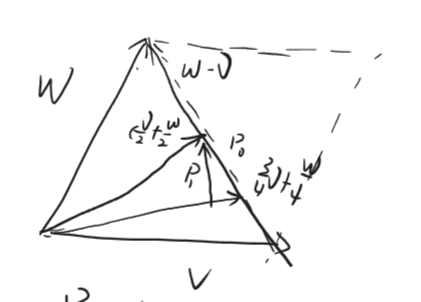
\includegraphics[width=\linewidth ,totalheight=0.95\textheight , keepaspectratio]{线性代数引论问题集1_1_15.png}
\caption{线性代数引论问题集1.1.15}
\end{figure}

已知该对角线为 $\boldsymbol{w} - \boldsymbol{v}$,标记该向量为 $P_0$,现在假定$\frac{3}{4}\boldsymbol{v} + \frac{1}{4}\boldsymbol{w}$ 射出去之后并没有落在对角线上,从而根据$\frac{1}{2}\boldsymbol{v} + \frac{1}{2}\boldsymbol{w}$ 和$\frac{3}{4}\boldsymbol{v} + \frac{1}{4}\boldsymbol{w}$ 的终点确立向量 $P_1$。

\begin{align*}
P_1 &= \frac{v}{2} + \frac{w}{2} - (\frac{3v}{4} + \frac{w}{4}) \\
    &= -\frac{1}{4}v + \frac{w}{4} \\
    &= \frac{1}{4}(w-v) \\    
 => P_1 // P_0
\end{align*}

因为 $\frac{1}{2}\boldsymbol{v} + \frac{1}{2}\boldsymbol{w}$ 在那条对角线的上,所以 $\frac{3}{4}\boldsymbol{v} + \frac{1}{4}\boldsymbol{w}$ 一定在这条对角线上。上面的证明过程还证明了 $P_1$ 的长度是1/4对角线长度,其终点位置刚好是对角线下面1/4的位置。





\backmatter
\chapter*{参考资料}
\addchtoc{参考资料}
\begin{thebibliography}{99}
\bibitem[线性代数引论]{线性代数引论} 《Introduction to Linear Algebra 5e》 by Gilbert Strang at 2016 .


\end{thebibliography}


\end{document}


